% To rebuild the .pdf from this source, use something like the following
%	latex quickref.tex
%	dvips -t letter -f -Pcmz < quickref.dvi >| quickref.ps
%	ps2pdf -sPAPERSIZE=letter quickref.ps

% german version (de)

\documentclass[12pt]{article}
\usepackage[latin1]{inputenc}
\usepackage{lscape}
\usepackage{setspace}
\usepackage{graphicx}
\usepackage{multicol}
\usepackage[normalem]{ulem}
\usepackage[english]{babel}
\usepackage{color}
\usepackage{hyperref}

\textheight=9in
\textwidth=7.5in
\headheight=0pt
\headsep=0pt
\topmargin=0in
\oddsidemargin=-0.4in
\evensidemargin=-0.6in
\parindent=0pt
\parsep=1pt
\pagestyle{empty}

\date {}

\makeatother

\begin{document}
	\begin{landscape}

%	\textit{Dan Kuester's all-leather}

	\begin{center}
	\begin{minipage}[m]
		{1in}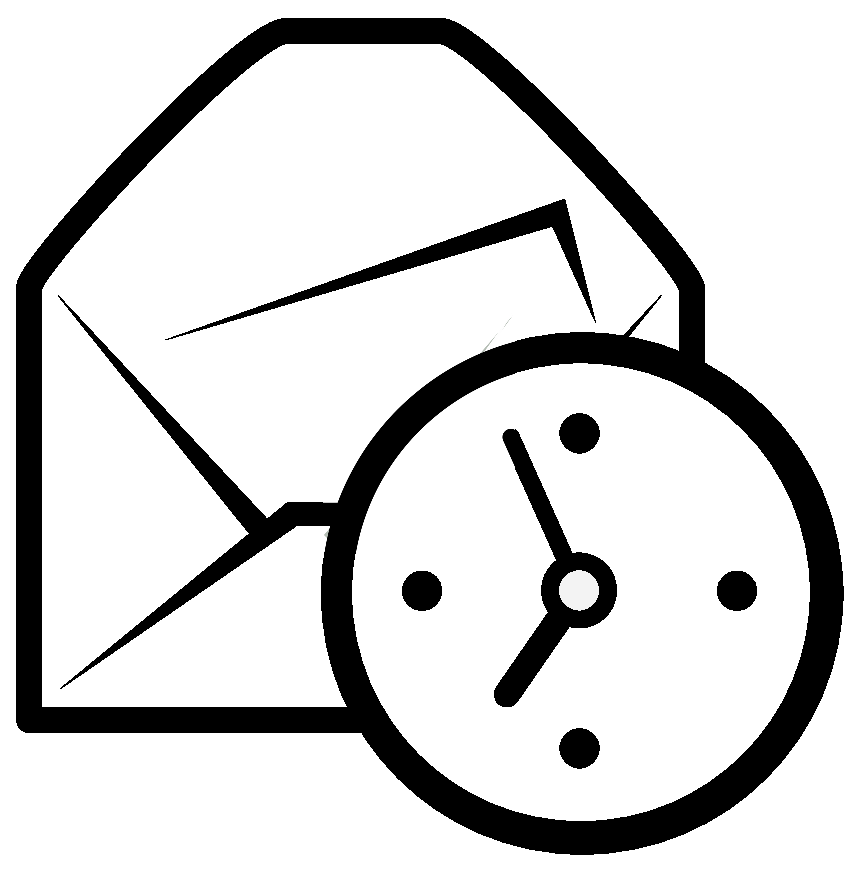
\includegraphics[height=0.9in]{../evolution-logo.eps}\hspace{5mm}
	\end{minipage}
	\hspace{5mm}
	\textbf{\Huge{Evolution-Kurzreferenz}}
	\end{center}

	\begin{center}
	\begin{multicols}{2}
	\section*{Allgemein}
	\begin{tabular*}{4in}{rp{1.5in}}
		\textit{\textbf{Komponenten}}		&					\\
		E-Mail					& \textbf{Strg+1}			\\
		Kontakte				& \textbf{Strg+2}			\\
		Kalender				& \textbf{Strg+3}			\\
		Aufgaben				& \textbf{Strg+4}			\\
		\vspace{1.5mm}
		Notizen					& \textbf{Strg+5}			\\
		\textit{\textbf{Befehle}}		&					\\
		Neuen Eintrag erstellen			& \textbf{Strg+N}			\\
		Zwischen den Fl�chen wechseln		& \textbf{F6}				\\
		Suchbegriff verwerfen			& \textbf{Shift+Strg+Q}			\\
		Fenster schlie�en			& \textbf{Strg+W}			\\
		Neues Fenster �ffnen			& \textbf{Shift+Strg+W}			\\
		\vspace{1.5mm}
		Evolution beenden			& \textbf{Strg+Q}			\\
		\textit{\textbf{Auswahl}}		&					\\
		Auswahl drucken				& \textbf{Strg+P}			\\
		Auswahl speichern			& \textbf{Strg+S}			\\
		Auswahl l�schen				& \textbf{Entf} oder \textbf{Backspace}	\\
		E-Mail/Kontakte in Ordner verschieben	& \textbf{Shift+Strg+V}			\\
		E-Mail/Kontakte in Ordner kopieren	& \textbf{Shift+Strg+Y}			\\
	\end{tabular*}
	\section*{Kontakte/Notizen}
	\begin{tabular*}{4in}{rp{1.5in}}
		\textit{\textbf{Allgemeine Befehle}}	&					\\
		Neuer Kontakt				& \textbf{Shift+Strg+C}			\\
		Neue Kontaktliste			& \textbf{Shift+Strg+L}			\\
		Neue Notiz				& \textbf{Shift+Strg+O}			\\
	\end{tabular*}
%	{\\ \vspace{5mm} \footnotesize \textit{* denotes the feature may not be implemented yet}}
	\section*{E-Mail}
	\begin{tabular*}{4in}{rp{1.5in}}
		\textit{\textbf{Allgemeine Befehle}}	&					\\
		Neue Nachricht				& \textbf{Shift+Strg+M}			\\
		\vspace{1.5mm}
		Nachrichten verschicken/abrufen		& \textbf{F9}				\\
		\textit{\textbf{Auswahl}}		&					\\
		Filter anwenden				& \textbf{Strg+Y}			\\
		In einem neuen Fenster �ffnen		& \textbf{Enter} oder \textbf{Strg+O}	\\
		\vspace{1.5mm}
		Auswahl weiterleiten			& \textbf{Strg+F}			\\
		\textit{\textbf{Nachrichtenlistenfeld}}	&					\\
		N�chste ungelesene Nachricht		& \textbf{.} oder \textbf{]}		\\
		\vspace{1.5mm}
		Vorherige ungelesene Nachricht		& \textbf{,} oder \textbf{[}		\\
		\textit{\textbf{Vorschaufeld}}		&					\\
		Antwort an Absender			& \textbf{Strg+R}			\\
		Antwort an Liste			& \textbf{Strg+L}			\\
		Antwort an alle		 		& \textbf{Shift+Strg+R}			\\
		Nach oben rollen			& \textbf{Backspace}			\\
		Nach unten rollen			& \textbf{Leertaste}			\\
	\end{tabular*}
	\section*{Kalender/Aufgaben}
	\begin{tabular*}{4in}{rp{1.5in}}
		\textit{\textbf{Allgemeine Befehle}}	&					\\
		Neuer Termin				& \textbf{Shift+Strg+A}			\\
		Neue Besprechung			& \textbf{Shift+Strg+E}			\\
		\vspace{1.5mm}
		Neue Aufgabe				& \textbf{Shift+Strg+T}			\\
%		\vspace{1.5mm}
%		Expunge/Purge old schedules		& \textbf{Strg+E}			\\
		\textit{\textbf{Navigation}}		&					\\
		Heute w�hlen				& \textbf{Strg+T}			\\
		Datum w�hlen				& \textbf{Strg+G}			\\
	\end{tabular*}
	\end{multicols}
	\end{center}
	\end{landscape}
 \end{document}
